\resizebox{0.55\columnwidth}{!}{
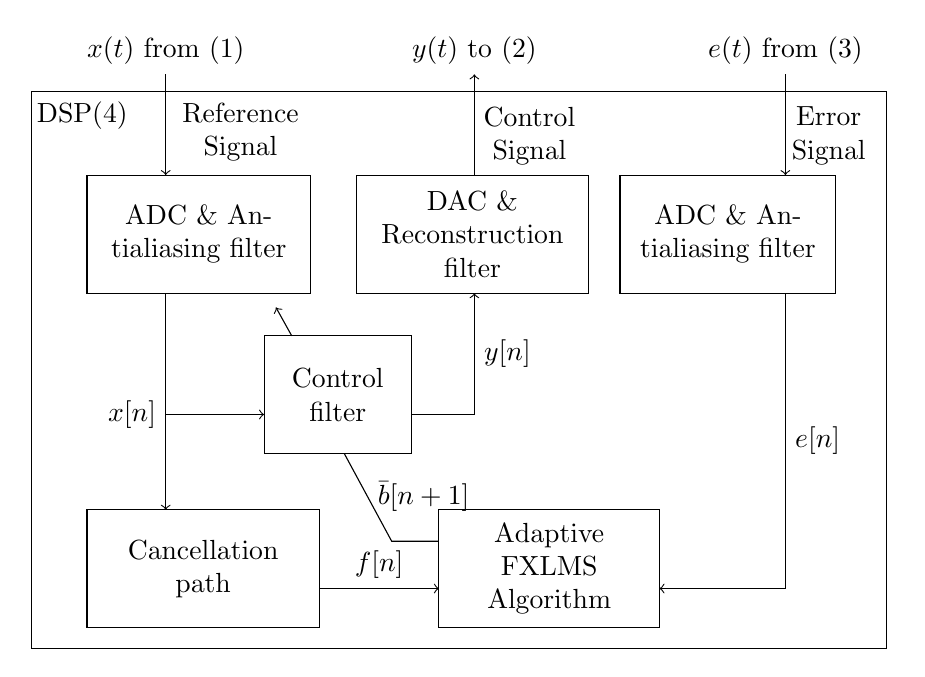
\begin{tikzpicture}
\draw  (-4,4.93) rectangle node[text width=2.5cm,align=center] {ADC \& Antialiasing filter} (-1.16,3.43);
\draw  (-4,0.68) rectangle node[text width=2.5cm,align=center] {Cancellation \\ path}(-1.05,-0.82);
\draw  (0.47,0.68) rectangle node[text width=2.5cm,align=center] {Adaptive FXLMS Algorithm} (3.27,-0.82);

\draw  (-1.75,2.89) rectangle node[text width=1.5cm,align=center,fill=white] {Control filter} (0.12,1.39);
\draw  (-0.58,4.93) rectangle node[text width=2.5cm,align=center] {DAC \& \\ Reconstruction filter}(2.37,3.43);
\draw  (2.77,4.93) rectangle node[text width=2.5cm,align=center] {ADC \& Antialiasing filter}(5.51,3.43);

\draw  (-4.71,5.99) rectangle (6.15,-1.08);
\node at (-4.06,5.69) {DSP(4)};
\node [text width=2cm,align=center] at (-2.05,5.48) {Reference Signal};

\draw[->] (-1.05,-0.32) -- node[above]{$f[n]$} (0.47,-0.32);

\draw[->] (4.87,3.43) -- node[right]{$e[n]$} (4.87,-0.32)  -- (3.27,-0.32);

\draw [->](4.87,6.21) node[above]{$e(t)$ from (3)} -- (4.87,4.93) ;
\draw [->](0.92,4.93)  --  (0.92,6.21) node[above]{$y(t)$ to (2)};
\draw [->](-3,3.43) -- (-3,0.68);

\draw [->](-3,1.89) node[left]{$x[n]$} -- (-1.75,1.89);

\draw[->] (0.12,1.89) -- (0.92,1.89) --node[right]{$y[n]$} (0.92,3.43);
\draw [->](-3,6.21) node[above]{$x(t)$ from (1)} -- (-3,4.93);
\node [text width=2cm,align=center] at (1.62,5.43) {Control Signal};
\node [text width=1.5cm,align=center] at (5.42,5.43) {Error Signal};

\draw (0.47,0.28) -- (-0.13,0.28) --node[above=0.25,right]{$\bar{b}[n+1]$} (-0.73,1.39);
\draw [->](-1.4,2.89) -- (-1.6,3.25);
\end{tikzpicture}}